\documentclass[14pt, titlepage, a4paper]{extarticle} %comment
\usepackage{fancyvrb}
\usepackage[utf8]{inputenc}
\usepackage[T2A]{fontenc}
\usepackage[russian]{babel}
\usepackage{amssymb, amsfonts}
\usepackage{amsmath}

\usepackage{graphicx}

\usepackage{lipsum}
\usepackage{style}
\textwidth 16cm
\textheight 25cm
\oddsidemargin -2.5mm
\evensidemargin -3mm
\topmargin -20mm
\parindent 1.25cm

\usepackage{xcolor}
\usepackage{hyperref}
% Цвета для гиперссылок
\definecolor{linkcolor}{HTML}{799B03} % цвет ссылок
\definecolor{urlcolor}{HTML}{000000} % цвет гиперссылок
\hypersetup{pdfstartview=FitH,  linkcolor=linkcolor,urlcolor=urlcolor, colorlinks=true}


\usepackage{comment}
%\usepackage{autonum}
\usepackage{amsthm}
\newtheorem{theorem}{Теорема}
\newtheorem{definition}{Определение}
\newtheorem{corollary}{Следствие}
\newtheorem{lemma}{Лемма}

\begin{document}
	
	%%%%%%%%%%%%%%%%%%%%PAGE%1%%%%%%%%%%%%%%%%%%%%
	%%%%%%%%%%%%%%%%%%%Вкладка%%%%%%%%%%%%%%%%%%%%
	
	\begin{center}
		ЗАДАНИЕ НА КУРСОВОЙ ПРОЕКТ\\
		по дисциплине «Численные методы»
	\end{center}
	
	~\\	
	Ф.И.О. \uline{\vspace{10pt} Бобров И.И., Игнатьев М.В., Абдуллаев Т.М.~~~~~~~~~~~}\\
	~\\
	~\\
	ТЕМА курсового проекта
	
	~\\
	Рекуррентные формулы и интегрирование по Ромбергу.
	\\
	~\\
	~\\
	ФОРМУЛИРОВКА  задания:
	
	\begin{itemize}
		\item Создать алгоритм решения поставленной задачи, реализовать его, протестировать программы;
		\item Оформить и представить итоги проделанной работы в виде отчета;
		\item Сформулировать выводы по полученным решениям, отметить достоинства и недостатки методов.
	\end{itemize}

	~\\
	РУКОВОДИТЕЛЬ проекта\uline{\hspace{80pt}}/ Пак Т.В./\\	
	\\
	~\\
	ДАТА ВЫДАЧИ задания\uline{~6~ноября~2021~}\\
	\\
	~\\
	СРОК ВЫПОЛНЕНИЯ задания 09.11.2020 – 10.01.2021\\
	\\
	~\\
	Задание получил \uline{Бобров И.И., Игнатьев М.В., Абдуллаев Т.М.}\\
	
	\thispagestyle{empty}
	\newpage
	
	%%%%%%%%%%%%%%%%%%%%PAGE%2%%%%%%%%%%%%%%%%%%%%
	%%%%%%%%%%%%%%%%%%Титульник%%%%%%%%%%%%%%%%%%%
	
	%\begin{comment}
	\fefutitlepage{Б8118-01.03.02миопд}{Бобров И.И.}{Игнатьев М.В.}{Абдуллаев Т.М.}{5}
	\defaultfont
	%\end{comment}

	%%%%%%%%%%%%%%%%%%%%PAGE%3%%%%%%%%%%%%%%%%%%%%
	%%%%%%%%%%%%%%%%%%Содержание%%%%%%%%%%%%%%%%%%

	\tableofcontents
	\pagebreak
	
	%%%%%%%%%%%%%%%%%%%%PAGE%4%%%%%%%%%%%%%%%%%%%%
	%%%%%%%%%%%%%%%%%%%Введение%%%%%%%%%%%%%%%%%%%
	
	\section*{Введение}
	\addcontentsline{toc}{section}{Введение}
	
	Объектом исследования являются численные методы решения задач численного интегрирования.\\
	\textit{Цель работы} – ознакомиться с рекуррентными формулами и методами интегрирования, решить предложенные типовые задачи, сформулировать выводы по полученным решениям, отметить достоинства и недостатки методов, приобрести практические навыки и компетенции, а также опыт самостоятельной профессиональной деятельности, а именно:
	\begin{itemize}
		\item создать алгоритм решения поставленной задачи и реализовать его, протестировать программы;
		\item освоить теорию вычислительного эксперимента; современных компьютерных технологий; 
		\item приобрести навыки представления итогов проделанной работы в виде отчета, оформленного в соответствии с имеющимися требованиями, с привлечением современных средств редактирования и печати.	
	\end{itemize}
	Работа над курсовым проектом предполагает выполнение следующих задач:
	\begin{itemize}
		\item дальнейшее углубление теоретических знаний обучающихся и их систематизацию;
		\item получение и развитие прикладных умений и практических навыков по направлению подготовки;
		\item овладение методикой решения конкретных задач;
		\item развитие навыков самостоятельной работы;
		\item развитие навыков обработки полученных результатов, анализа и осмысления их с учетом имеющихся литературных данных;
		\item приобретение навыков оформления описаний программного продукта;
		\item повышение общей и профессиональной эрудиции.
	\end{itemize}

	
	\pagebreak
	
	%%%%%%%%%%%%%%%%%%%%PAGE%5%%%%%%%%%%%%%%%%%%%%
	%%%%%%%%%%%%%%%%Основная%часть%%%%%%%%%%%%%%%%
	%%%%%%%%%%%%%%%Постановка%задачи%%%%%%%%%%%%%%%
	
	\section*{Основная часть}
	\addcontentsline{toc}{section}{Основная часть}
	
	\subsection*{Рекуррентные формулы}
	\addcontentsline{toc}{subsection}{Рекуррентные формулы.}
	
	Приближения имеют высокую точность, если использовать большее количество подынтервалов. Сколько их следует выбрать? Ответить на этот вопрос может помочь процесс последовательного
	выбора двух, четырех и т. д. подынтервалов, пока не будет достигнута требуемая точность. Сначала необходимо сгенерировать последовательность {$T(J)$} формул трапеций для приближений. Как только число подынтервалов удваивается, число значений функции также приблизительно удваивается, поскольку функцию нужно вычислять во всех предыдущих точках и во всех средних точках предыдущих подынтервалов (рис 1). В теореме 7.4 объясняется, как удалить лишние вычисления функции и сложения.
	
	\begin{figure}[h]
		\centering
		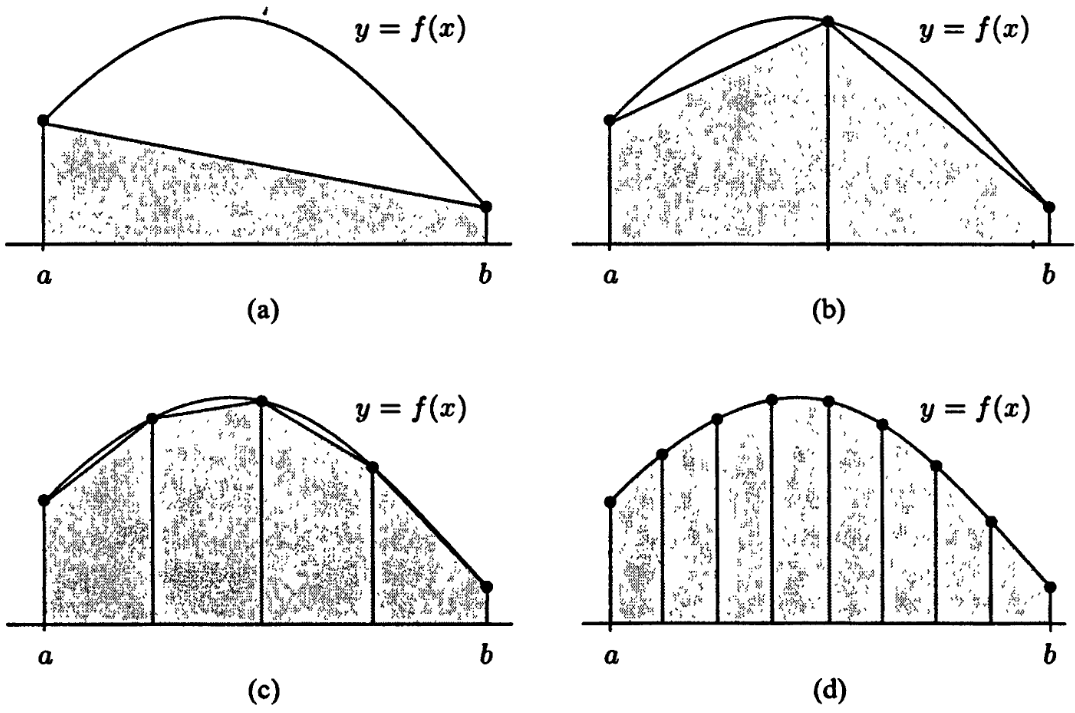
\includegraphics[width=400pt]{pic1.png}
		\caption{\textbf{(a)} $T(0)$ — площадь под $2^0 = 1$ трапецией, \textbf{(b)} $T(1)$ — площадь под		$2^1 = 2$ трапециями, \textbf{(с)} $Т(2)$ — площадь под $2^2 = 4$ трапециями, \textbf{(d)} $Г(3)$ — площадь под $2^3 = 8$ трапециями}
	\end{figure}
	
	\begin{theorem}\label{th:7.4}
		\textbf{(последовательные формулы трапеций).} Предположим, что $J \geqslant 1$ и точки \{$x_k = a + kh$\} делят интервал $\left[a; b\right]$ на $2^J = 2M$ подынтервалов с одинаковым шагом $h = (b-a)/2^J$. Формулы трапеций $T(f,h)$ и $T(f,2h)$ удовлетворяют соотношению
		\begin{equation}\label{eq:1}
			T(f,h)=\frac{T(f,2h)}{2} + h\sum_{k=1}^{M}f(x_{2k-1})
		\end{equation}
	\end{theorem}
	
	\begin{definition}\label{df:7.3}
		\textbf{(последовательность формул трапеций).} Определим $T(0) = (h/2)(f(a)+f(b))$ как формулу трапеций с шагом длины $h = b - a$. Затем для каждого $J\ge1$ определим $T(J)=T(f,h)$, где $T(f,h)$ - формула трапеций с шагом длинны $h = (b-a)/2$.
	\end{definition}
	
	\begin{corollary}\label{cr:7.4}
	\textbf{(рекуррентная формула трапеций).} Начнем с $Т(0) = (h/2) х (f(a) + f(b))$. Тогда последовательность формул трапеций ${T(J)}$ генерируется согласно рекуррентной формуле
		\begin{equation}\label{eq:2}
			T(J) = \frac{T(J-1)}{2}+ h\sum_{k-1}^{M}f(x_{2k-1})~~\text{для}~J = 1, 2,~...~.
		\end{equation}
	где $h=(b-a)/2^J$ и ${x_k = a + kh}$.
	\end{corollary}
	
	
	\begin{theorem}\label{th:7.5}
		\textbf{(рекуррентная формула Симпсона).} Предположим, что $\{T(J)\}$ - последовательность формул трапеций, сгенерированная согласно следствию (\ref{cr:7.4}). Если $J\ge1$ и $S(J)$ - формула Симпсона для $2^J$ подынтервалов $[a;b]$, то $S(J)$ и формулы трапеций $T(J-1)$ и $T(J)$ удовлетворяют соотношению
		\begin{equation}\label{eq:7}
			S(J) = \frac{4T(J)-T(J-1)}{3}~~~\text{для}~J = 1,2,~...~.
		\end{equation}
	\end{theorem}
	
	
	\begin{theorem}\label{th:7.6}
		\textbf{(рекуррентная формула Буля).} Предположим, что $\{S(J)\}$ - последовательность формул Симпсона, сгенерированная согласно теореме (\ref{th:7.5}). Если $J\ge2$ и $B(J)$ - формула Буля для $2^J$ подынтервалов интервала $[a;b]$, то $B(J)$ и формулы Симпсона $S(J-1)$ и $S(J)$ удовлетворяют соотношению
		\begin{equation}\label{eq:14}
			B(J) = \frac{16S(J)-S(J-1)}{15}~~~\text{для}~J=2,3,~...~.
		\end{equation}
	\end{theorem}
	%%%%%%%%%%%%%%%%%%%%%%%%%%%%%%%%%%%%%%%%%%%%%%%%%%%%%%%%%%%%%%%%%%%%%%%%%%%%%%%%%%%%%%%
	~\\
	\subsection*{Интегрирование по Ромбергу}
	\addcontentsline{toc}{subsection}{Интегрирование по Ромбергу}
	
	Предположим, что формула приближения используется с шагами длины h и 2Л. Воспользуемся алгебраическими преобразованиями двух ответов, чтобы получить уточненный ответ. Каждый последующий уровень улучшения увеличивает порядок остаточного члена с $O(h^{2N})$ до $O(h^{2N+2})$. Этот процесс, называемый интегрированием по Ромбергу.
	\begin{eqnarray}
		\nonumber
		\int_{a}^{b}{f(x)dx} &=& T(f,h)+O(h^2),
		\nonumber
		\cr \int_{a}^{b}{f(x)dx} &=& S(f,h)+O(h^4),
		\nonumber
		\cr \int_{a}^{b}{f(x)dx} &=& B(f,h)+O(h^6).
	\end{eqnarray}
	~\\
	
	\begin{lemma}
		\textbf{(улучшение Ричардсона для интегрирования по Ромбергу).} Заданы два приближения, $R(2h,К-1)$ и $R(h,K-1)$, для величины $Q$, которые
		удовлетворяют равенствам
		\begin{equation}\label{eq:28}
			Q = R(h,K-1)+c_1h^{2K}+c_2h^{2K+2}+...
		\end{equation}
		и
		\begin{equation}\label{eq:29}
			Q = R(2h,K-1)+c_14^Kh^{2K}+c_24^{K+1}h^{2K+2}+...~.
		\end{equation}
		Улучшенное приближение имеет вид
		\begin{equation}\label{eq:30}
			Q = \frac{4^KR(h,K-1)-R(2h,K-1)}{4^K-1}+O(h^{2K+2}).
		\end{equation}
	\end{lemma}


	\begin{definition}\label{df:7.4}
		Определим последовательность ${R(J,K):J\ge K}^{\infty}_{J=0}$ формул квадратуры для $f(x)$ на интервале $[a;b]$ следующим образом.
		\begin{eqnarray}
			\nonumber
			R(J,0) &=& T(J)~~~\text{для}~J\ge 0\text{, последовательная формула трапеций.}\\
			\nonumber
			R(J,1) &=& S(J)~~~\text{для}~J\ge 1\text{, последовательная формула Симпсона.}\\
			\label{eq:31}
			R(J,2) &=& B(J)~~~\text{для}~J\ge 2\text{, последовательная формула Буля.}
		\end{eqnarray}
	\end{definition}
	~\\
	Общей формулой построения улучшения
	\begin{equation}\label{eq:33}
		R(J,K) = \frac{4^KR(J,K-1)-R(J-1,K-1)}{4^K-1}~~~\text{для}~~J\ge K.
	\end{equation}
	
	\begin{theorem}\label{th:7}
		\textbf{(точность интегрирования по Ромбергу).} Предположим, что $f \in C^{2K+2}[a;b]$. Тогда ошибка усечения для приближения Ромберга задается формулой
		\begin{equation}\label{eq:34}
			\int_{a}^{b}{f(x)dx} = R(J,K) + b_Kh^{2K+2}f^{(2K+2)}(c_{J,K}) = R(J,K) + O(h^{2K+2}),
		\end{equation}	
		где $h = (b-a)/2^J,~b_K$ - постоянная, зависящая от $K$, и $c_{J,K}\in[a;b].$
	\end{theorem}
	
	
	~\\
	\subsection*{Квадратура Буля}
	\addcontentsline{toc}{subsection}{Квадратура Буля}
	
	\begin{equation}
	\nonumber
	\int_{a}^{b}{f(x)dx} = \frac{(b-a)}{90}\cdot(7y_0+32y_1+12y_2+32y_3+7y_4)
	\end{equation}
	Как мы ее получили?\\
	Построим полином Лагранжа 4ой степени от $f(x)$, посчитаем аналитически интеграл от этого полинома, полученный результат и будет квадратурой Буля.
	
	\[h = \frac{b-a}{4} \]
	\[x_i = a + i \cdot h = a + i\cdot \frac{b - a}{4} \]
	\[L_4(x) = l_0(x)y_0 + l_1(x)y_1 + l_2(x)y_2 + l_3(x)y_3 + l_4(x)y_4 \]
	Построим базисные полиномы к полиному Лагранжа:
	\[l_0(x) = \frac{(x - x_1)(x - x_2)(x - x_3)(x - x_4)}{(x_0 - x_1)(x_0 - x_2)(x_0 - x_3)(x_0 - x_4)} = \]
	\[ = \frac{(x - a - h)(x - a - 2h)(x - a - 3h)(x - a - 4h)}{24h^4} \]
	\[l_1(x) = \frac{(x - x_0)(x - x_2)(x - x_3)(x - x_4)}{(x_1 - x_0)(x_1 - x_2)(x_1 - x_3)(x_1 - x_4)} =\]
	\[ = -\frac{(x - a)(x -a - 2h)(x - a - 3h)(x - a - 4h)}{6h^4} \]
	\[l_2(x) = \frac{(x - x_0)(x - x_1)(x - x_3)(x - x_4)}{(x_2 - x_0)(x_2 - x_1)(x_2 - x_3)(x_2 - x_4)} = \]
	\[= \frac{(x - a)(x - a - h)(x - a - 3h)(x - a - 4h)}{4h^4} \]
	\[l_3(x) = \frac{(x - x_0)(x - x_1)(x - x_2)(x - x_4)}{(x_3 - x_0)(x_3 - x_1)(x_3 - x_2)(x_3 - x_4)} = \]
	\[= -\frac{(x - a)(x - a - h)(x - a - 2h)(x - a - 4h)}{6h^4} \]
	\[l_4(x) = \frac{(x - x_0)(x - x_1)(x - x_2)(x - x_3)}{(x_4 - x_0)(x_4 - x_1)(x_4 - x_2)(x_4 - x_3)} = \]
	\[= \frac{(x - a)(x - a - h)(x - a - 2h)(x - a - 3h)}{24h^4} \]
	Проинтегрируем базисные полиномы:
	\[\int_{a}^{b}{l_0(x)\,dx} = \int_{a}^{b}{\frac{(x - a - h)(x - a - 2h)(x - a - 3h)(x - a - 4h)}{24h^4}\,dx} = \frac{7}{90}(b-a) \]
	\[\int_{a}^{b}{l_1(x)\,dx} = \int_{a}^{b}{-\frac{(x - a)(x -a - 2h)(x - a - 3h)(x - a - 4h)}{6h^4}\,dx} = \frac{16}{45}(b-a) \]
	\[\int_{a}^{b}{l_2(x)\,dx} = \int_{a}^{b}{\frac{(x - a)(x - a - h)(x - a - 3h)(x - a - 4h)}{4h^4}\,dx} = \frac{2}{15}(b-a) \]
	\[\int_{a}^{b}{l_3(x)\,dx} = \int_{a}^{b}{-\frac{(x - a)(x - a - h)(x - a - 2h)(x - a - 4h)}{6h^4}\,dx} = \frac{16}{45}(b-a) \]
	\[\int_{a}^{b}{l_4(x)\,dx} = \int_{a}^{b}{\frac{(x - a)(x - a - h)(x - a - 2h)(x - a - 3h)}{24h^4}\,dx} = \frac{7}{90}(b-a) \]
	Тогда интеграл от полинома Лагранжа будет следующим:
	\[\int_{a}^{b}{L_4(x)\,dx} = y_0\int_{a}^{b}{l_0(x)\,dx} + y_1\int_{a}^{b}{l_1(x)\,dx} +\] \[ + y_2\int_{a}^{b}{l_2(x)\,dx} + y_3\int_{a}^{b}{l_3(x)\,dx} + y_4\int_{a}^{b}{l_4(x)\,dx} = \]
	\[= \frac{7}{90}(b-a)\cdot y_0 + \frac{16}{45}(b-a)\cdot y_1 + \frac{2}{15}(b-a)\cdot y_2 + \frac{16}{45}(b-a)y_3 + \frac{7}{90}(b-a)\cdot y_4 = \]
	\[= (b - a) \cdot \left(\frac{7}{90}\cdot y_0 + \frac{16}{45}\cdot y_1 + \frac{2}{15}\cdot y_2 + \frac{16}{45} \cdot y_3 + \frac{7}{90} \cdot y_4 \right) \]
	Домножим полученное выражение на $\frac{90}{90}$ и получим квадратурную формулу Буля:
	\[\int_{a}^{b}{f(x)\,dx} = \frac{(b - a)}{90} \cdot \left(7y_0 + 32y_1 + 12y_2 + 32y_3 + 7y_4 \right) \]
	
	%\subsubsection*{Описание алгоритмов решения}
	%\addcontentsline{toc}{subsubsection}{Описание алгоритмов решения}
	
	\pagebreak
	\subsection*{Вычислительный эксперимент}
	\addcontentsline{toc}{subsection}{Вычислительный эксперимент}
	
	В данных экспериментах интеграл вычисляется не с заданной точностью, а с разными интервалами ($n = 2^{J}$, $J$ - параметр в рекуррентных формулах)\vspace{5pt}\\
	\subsubsection*{Эксперимент 1}
	\addcontentsline{toc}{subsubsection}{Эксперимент 1}

	\[\int_{1}^{5} \frac{dx}{x} = 1.609437912\]
	Ответ по рекуррентной формуле трапеций:
	\[T(0) = 2.4000000000, \Delta T(0) = 0.7905620880\]
	\[T(1) = 1.8666666667, \Delta T(1) = 0.2572287547\]
	\[T(2) = 1.6833333333, \Delta T(2) = 0.0738954213\]
	\[T(3) = 1.6289682540, \Delta T(3) = 0.0195303420\]
	Ответ по рекуррентной формуле Симпсона:
	\[S(1) = 1.6888888889, \Delta S(1) = 0.0794509769\]
	\[S(2) = 1.6222222222, \Delta S(2) = 0.0127843102\]
	\[S(3) = 1.6108465608, \Delta S(3) = 0.0014086488\]
	Ответ по рекуррентной формуле Буля:
	\[B(2) = 1.6177777778, \Delta B(2) = 0.0083398658\]
	\[B(3) = 1.6100881834, \Delta B(3) = 0.0006502714\]
	Ответ по методу Ромберга:
	\[R(5, 5) = 1.6094381258, \Delta R(5, 5) = 0.0000002138\]
	\subsubsection*{Эксперимент 2}
	\addcontentsline{toc}{subsubsection}{Эксперимент 2}
	\[\int_{-0.75}^{0.75}\cos(x)dx \approx 1.363277520\]
	Ответ по рекуррентной формуле трапеций:
	\[T(0) = 1.0975333033,\quad \Delta T(0) = 0.2657442167\]
	\[T(1) = 1.2987666517,\quad \Delta T(1) = 0.0645108683\]
	\[T(2) = 1.3472640423,\quad \Delta T(2) = 0.0160134777\]
	\[T(3) = 1.3592812008,\quad \Delta T(3) = 0.0039963192\]
	Ответ по рекуррентной формуле Симпсона:
	\[S(1) = 1.3658444344,\quad \Delta S(1) = 0.0025669144\]
	\[S(2) = 1.3634298391,\quad \Delta S(2) = 0.0001523191\]
	\[S(3) = 1.3632869203,\quad \Delta S(3) = 0.0000094003\]
	Ответ по рекуррентной формуле Буля:
	\[B(2) = 1.3632688661,\quad \Delta B(2) = 0.0000086539\]
	\[B(3) = 1.3632773923,\quad \Delta B(3) = 0.0000001277\]
	Ответ по методу Ромберга:
	\[R(5, 5) = 1.3632775200,\quad \Delta R(5,5) = 0.0000000000\]
	\subsubsection*{Эксперимент 3}
	\addcontentsline{toc}{subsubsection}{Эксперимент 3}
	
	\[\int_{0}^{\frac{\pi}{2}}\left(x^2 + x + 1\right)\cos(x)dx \approx 2.038197427076\]
	Ответ по рекуррентной формуле трапеций:
	\[T(0) = 0.7853981634,\quad \Delta T(0) = 1.2527992637\]
	\[T(1) = 1.7268126568,\quad \Delta T(1) = 0.3113847703\]
	\[T(2) = 1.9605341666,\quad \Delta T(2) = 0.0776632605\]
	\[T(3) = 2.0187939481,\quad \Delta T(3) = 0.0194034790\]
	Ответ по рекуррентной формуле Симпсона:
	\[S(1) = 2.0406174879,\quad \Delta S(1) = 0.0024200608\]
	\[S(2) = 2.0384413365,\quad \Delta S(2) = 0.0002439094\]
	\[S(3) = 2.0382138752,\quad \Delta S(3) = 0.0000164482\]
	Ответ по рекуррентной формуле Буля:
	\[B(2) = 2.0382962597,\quad \Delta B(2) = 0.0000988327\]
	\[B(3) = 2.0381987112,\quad \Delta B(3) = 0.0000012841\]
	Ответ по методу Ромберга:
	\[R(5, 5) = 2.0381974271,\quad \Delta R(5,5) = 0.0000000000\]
	
	В результате вычислительных экспериментов мы обнаружили что решение по методу Ромберга является очень точным.
	
	%%%%%%%%%%%%%%%%%%%%%%%%%%%%%%%%%%%%%%%%%%%%%%
	%%%%%%%%%%%%%%%%%%%%PAGE%?%%%%%%%%%%%%%%%%%%%%
	%%%%%%%%%%%%%%%%%%Заключение%%%%%%%%%%%%%%%%%%
	
	\section*{Заключение}
	\addcontentsline{toc}{section}{Заключение}
	
	В результате работы над курсовым проектом приобрел практические навыки владения:
	\begin{itemize}
		\item современными численными методами решения задач математической экономики;
		\item основами алгоритмизации для численного решения задач математической экономики на одном из языков программирования;
		\item инструментальными средствами, поддерживающими разработку программного обеспечения для численного решения задач математической экономики; 
	\end{itemize}
	а также навыками представления итогов проделанной работы в виде отчета, оформленного в соответствии с имеющимися требованиями, с привлечением современных средств редактирования и печати.
	
	\pagebreak

	%%%%%%%%%%%%%%%%%%%%PAGE%?%%%%%%%%%%%%%%%%%%%%
	%%%%%%%%%%%%%%%%%%%Источники%%%%%%%%%%%%%%%%%%
	
	\section*{Список используемых источников}
	\addcontentsline{toc}{section}{Источники}
	
	\textbf{Источники}
	\begin{enumerate}
		\item Численные методы. Использование Matlab. Третье издание. Джон Г. Мэтьюз Издательский дом $"$Вильямс$"$ 2001
		\item wikipedia Численное интегрирование\\ $\href{https://en.wikipedia.org/wiki/Numerical_integration}{https://en.wikipedia.org/wiki/Numerical_integration}$
		
		\item Documentation Python 3.6	
	\end{enumerate}
	
	\pagebreak
	
	%%%%%%%%%%%%%%%%%%%%PAGE%?%%%%%%%%%%%%%%%%%%%%
	%%%%%%%%%%%%%%%%%%Приложения%%%%%%%%%%%%%%%%%%
	
	\section*{Приложения}
	\addcontentsline{toc}{section}{Приложения}
	
	\subsection*{Реализация описанных методов на языке Python 3.6}
	\addcontentsline{toc}{subsection}{Реализация описанных методов на языке Python 3.6}
	
	\begin{Verbatim}[numbers=left,xleftmargin=0mm]
  import math
	
	
  def T(context, J):
    a, b, f = context['a'], context['b'], context['f']
    h = (b - a) / (2 ** J)
    if J == 0:
      return h * (f(a) + f(b)) / 2
    s = 0
    m = 2 ** (J - 1)
    for i in range(1, m + 1):
      s += f(a + (2 * i - 1) * h)
    return T(context, J - 1) / 2 + h * s


  def S(context, J):
    return (4 * T(context, J) - T(context, J - 1)) / 3


  def B(context, J):
    return (16 * S(context, J) - S(context, J - 1)) / 15


  def R(context, J, K):
    if K == 0:
      return T(context, J)
    if K == 1:
      return S(context, J)
    if K == 2:
      return B(context, J)
    return ((4**K)*R(context,J,K-1)-R(context,J-1,K-1))/(4**K-1)
	\end{Verbatim}
	
	\pagebreak	
	
	
\end{document}